\documentclass[a4paper,
fontsize=11pt,
%headings=small,
oneside,
numbers=noperiodatend,
parskip=half-,
bibliography=totoc,
final
]{scrartcl}

\usepackage{synttree}
\usepackage{graphicx}
\setkeys{Gin}{width=.6\textwidth} %default pics size

\graphicspath{{./plots/}}
\usepackage[ngerman]{babel}
\usepackage[T1]{fontenc}
%\usepackage{amsmath}
\usepackage[utf8x]{inputenc}
\usepackage [hyphens]{url}
\usepackage{booktabs} 
\usepackage[left=2.4cm,right=2.4cm,top=2.3cm,bottom=2cm,includeheadfoot]{geometry}
\usepackage{eurosym}
\usepackage{multirow}
\usepackage[ngerman]{varioref}
\setcapindent{1em}
\renewcommand{\labelitemi}{--}
\usepackage{paralist}
\usepackage{pdfpages}
\usepackage{lscape}
\usepackage{float}
\usepackage{acronym}
\usepackage{eurosym}
\usepackage[babel]{csquotes}
\usepackage{longtable,lscape}
\usepackage{mathpazo}
\usepackage[flushmargin,ragged]{footmisc} % left align footnote

\usepackage{listings}

\urlstyle{same}  % don't use monospace font for urls

\usepackage[fleqn]{amsmath}

%adjust fontsize for part

\usepackage{sectsty}
\partfont{\large}

%Das BibTeX-Zeichen mit \BibTeX setzen:
\def\symbol#1{\char #1\relax}
\def\bsl{{\tt\symbol{'134}}}
\def\BibTeX{{\rm B\kern-.05em{\sc i\kern-.025em b}\kern-.08em
    T\kern-.1667em\lower.7ex\hbox{E}\kern-.125emX}}

\usepackage{fancyhdr}
\fancyhf{}
\pagestyle{fancyplain}
\fancyhead[R]{\thepage}

%meta
%meta

\fancyhead[L]{Ch. Kahle \\ %author
LIBREAS. Library Ideas, 26 (2014). % journal, issue, volume.
\href{http://nbn-resolving.de/urn:nbn:de:kobv:11-100222672
}{urn:nbn:de:kobv:11-100222672}} % urn
\fancyhead[R]{\thepage} %page number
\fancyfoot[L] {\textit{Creative Commons BY 3.0}} %licence
\fancyfoot[R] {\textit{ISSN: 1860-7950}}

\title{\LARGE{Die Offene Bibliothek von Clegg \& Guttmann}} %title %title
\author{Christian Kahle} %author

\setcounter{page}{}

\usepackage[colorlinks, linkcolor=black,citecolor=black, urlcolor=blue,
breaklinks= true]{hyperref}

\date{}
\begin{document}

\maketitle
\thispagestyle{fancyplain} 

%abstracts

%body
\emph{Offene} oder \emph{Öffentliche Bücherschränke} und vergleichbare
Installationen, die dem freien Austausch von Büchern dienen, gehören
heute zum Alltagsbild vieler Städte. Auf der Plattform
\emph{OpenBookCase.org} sind mittlerweile mehr als 700 Projekte
verzeichnet, die sich überwiegend frei zugänglich im öffentlichen Raum
befinden. Die meisten dieser Mikroinstitutionen stellen Variationen
einer Kernidee dar, die sich auf die Projekte der Künstler \emph{Martin
Clegg} und \emph{Michael Guttmann} zurückführen lässt.

\section*{Die \emph{Offene
Bibliothek}}\label{die-offene-bibliothek}

Frei zugängliche Bücherbehältnisse installierte das Künstlerduo
\emph{Clegg \& Guttmann} 1991 an verschiedenen Standorten in Graz. In
der Zeitschrift des \emph{Grazer Kunstvereins} veröffentlichten die
Künstler einen theoretischen Entwurf zu ihrer Alternativbibliothek:

\begin{quote}
Eine Bibliothek ohne Bibliothekare und Überwachung, deren Bücherbestand
von den Benützern selbst durch ein Tauschsystem, demzufolge jedes
entliehene Buch nach Gutdünken des Benützers durch ein anderes zu
ersetzen ist, bestimmt wäre. (Clegg \& Guttmann 1990)
\end{quote}

Das Tauschsystem hebt die Rollenhierarchie zwischen dem Fachpersonal
einer Bibliothek und ihren Benutzern auf. Jeder Beteiligte ist
gleichermaßen Nutzer und Erneuerer des gemeinsamen Buchbestands. Die
Offenheit derartiger Bücherbehältnisse liegt nicht allein in ihrer
öffentlichen Zugänglichkeit begründet. In den englischsprachigen Texten
der Künstler fällt die doppelte Bestimmung als \emph{Open Public
Library} auf. Anlässlich einer späteren Realisierung ihrer \emph{Offenen
Bibliothek} stellten \emph{Clegg \& Guttmann} folgende Leitlinien auf:

\begin{quote}
\begin{enumerate}
\def\labelenumi{\arabic{enumi}.}
\itemsep1pt\parskip0pt\parsep0pt
\item
  Die \enquote{Offene Bibliothek} soll ohne Hierarchie auskommen.
\item
  Die \enquote{Offene Bibliothek} soll durch keinerlei Sicherheits- oder
  Kontrolleinrichtungen geschützt werden.
\item
  Den Nutzern werden keine zusätzlichen Bestimmungen auferlegt, die über
  die Definition der Bibliothek als einen Ort, an dem für einen
  begrenzten Zeitraum zu vergebendes Lesematerial zur Verfügung steht,
  hinausgehen.
\item
  Es werden keine Kriterien für eine Auswahl des Lesematerials
  festgelegt. (Clegg \& Guttmann, Bemerkungen zur Offenen Bibliothek,
  in: Könneke 1994, S. 28.)
\end{enumerate}
\end{quote}

Der gegebenen Minimaldefinition nach kann prinzipiell eine Vielzahl an
Orten, Behältnissen oder Installationen zu einer \emph{Offenen
Bibliothek} erklärt werden. Wie aber wird aus einer Menge an
zusammengetragenen Büchern ein Bestand und somit der Ort zu einer
Bibliothek? Mit der Etablierung spezifischer Formen der Nutzung durch
eine Nutzergemeinschaft, die sich im Zuge sozialer
Kommunikationsprozesse konstituiert:

\begin{quote}
Die Notwendigkeit, Normen für die ordnungsgemäße Benutzung der
Bibliothek zu erstellen, wird eine Diskussion über die Werte und Ziele
der Gemeinschaft erforderlich machen. Die Findung und Ausübung von
gewaltlosen Sanktionen gegen die Verletzung des richtigen Gebrauchs der
Bibliothek kann zu einer Übung in metaphorischer Selbstverwaltung
werden. (Clegg \& Guttmann 1990)
\end{quote}

Kurz sei hier auf den Diskurs über Gemeingüter verwiesen: Ist es
sinnvoll, den geteilten Buchbestand als \emph{Commons} und die damit
verbundenen Formen der Nutzung und Pflege als \emph{Commoning} zu
verstehen? Problematisch ist hier vielleicht die genaue Bestimmung des
Gemeinguts, da für die Nutzer kein konstanter Zugriff auf inhaltlich
bestimmte Wissensbestände garantiert werden kann.

\section*{Porträt einer
Gemeinschaft}\label{portruxe4t-einer-gemeinschaft}

Ursprünglich waren die \emph{Offenen Bibliotheken} als experimentelle
Modelle gedacht. Als temporäre Installationen sollte sich an ihnen
zeigen, in welcher Form die Anwohner auf ein derartiges Angebot
reagieren würden. Etwaige Plünderungen oder Beschädigungen stellten kein
Scheitern, sondern einen möglichen Verlauf des Experiments dar. Heute
werden die Projekte bewusst so geplant und gepflegt, dass sie für einen
längeren Zeitraum stabil und attraktiv bleiben. Dies führt jedoch zu
einer Einschränkung ihres basisdemokratischen Charakters.

Ausgehend von \emph{Marcel Duchamps} Entgrenzung des überkommenen
Kunstbegriffs werfen \emph{Clegg \& Guttmann} die Frage auf, inwiefern
ihre Installationen als Kunst verstanden werden können. Ein
\emph{Öffentlicher Bücherschrank} stellt einen zur kollektiven Nutzung
in den Außenraum verschobenen Gebrauchsgegenstand dar, an dem sich
soziale Prozesse manifestieren:

\begin{quote}
Eine solche Bibliothek könnte als Institution zu einer Selbstdefinition
der Gemeinschaft beitragen; sie würde ihre Lesegewohnheiten und
intellektuellen Vorlieben widerspiegeln und wäre damit eine Art Porträt
einer Gemeinschaft. (Ebd.)
\end{quote}

Für den Aufbau und Erhalt einer \emph{Offenen Bibliothek} wirken
verschiedene soziale Akteure zusammen, wofür \emph{Clegg \& Guttmann}
den von \emph{Joseph Beuys} geprägten Begriff der \emph{sozialen
Skulptur} aufgreifen. In Hamburg richteten die Künstler parallel zu
ihren Installationen ein gemeinsames Informations- und
Dokumentationszentrum ein, um eine Kommunikationsverbindung zwischen den
beteiligten Bevölkerungsgruppen zu schaffen:

\begin{quote}
Wir glauben, daß eine der wichtigsten Aufgaben von Kunst ist, Porträts
zu erzeugen, während über den Prozeß des Porträtierens selbst
reflektiert wird. {[}\ldots{}{]} Dieses Projekt ist von uns gedacht als
ein Porträt eines Stadtteils. Es wird den Leuten in den verschiedenen
Stadtteilen in sehr direkter Weise ermöglichen, ihren unmittelbaren
sozialen Kontext besser zu verstehen. Würde man es erweitern, könnte das
Projekt zu einem Porträt der Stadt Hamburg werden. (Clegg \& Guttmann
1993)
\end{quote}

Ein Porträt ist hier kein mit den Mitteln der Malerei geschaffenes
Kunstwerk statischer Referenz. Kunst besteht hier im Anbahnen und
Ermöglichen von Bewusstseins- und Kommunikationsprozessen.

\begin{figure}[htbp]
\centering
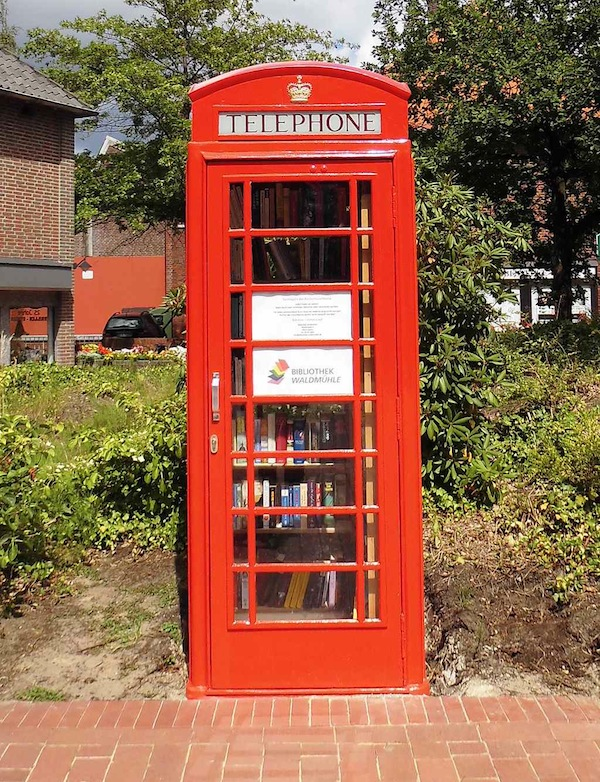
\includegraphics{img/BuchertauschborseSoltau.jpg}
\caption{Bildunterschrift: CC-BY-3.0,Urheber: ChristianSW,
\url{https://commons.wikimedia.org/wiki/File:B\%C3\%Bcchertauschb\%C3\%B6rse_Soltau.jpg}}
\end{figure}

\begin{figure}[htbp]
\centering
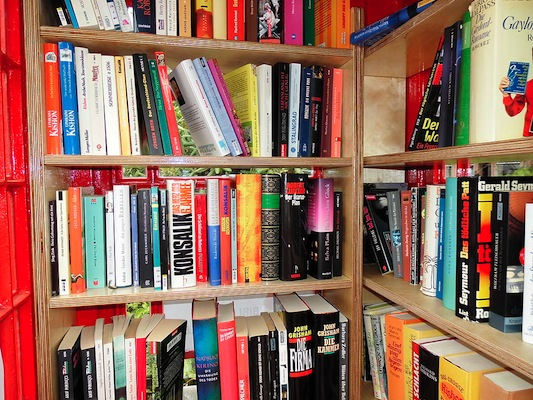
\includegraphics{img/BuchertauschborseSoltauII.jpg}
\caption{Bildunterschrift: CC-BY-3.0, Urheber: ChristianSW,
\url{https://commons.wikimedia.org/wiki/File:B\%C3\%BCchertauschb\%C3\%B6rse_Soltau_II.jpg}}
\end{figure}

\begin{figure}[htbp]
\centering
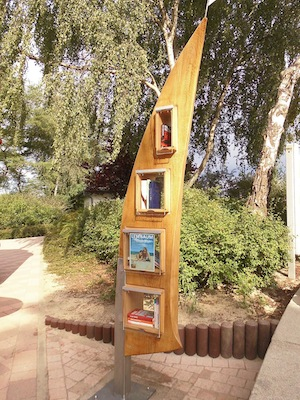
\includegraphics{img/LesebaumKarlshagen.jpg}
\caption{Bildunterschrift: CC-BY-3.0, Urheber: ChristianSW,
\url{https://commons.wikimedia.org/wiki/File:Lesebaum_Karlshagen.jpg}}
\end{figure}

\begin{figure}[htbp]
\centering
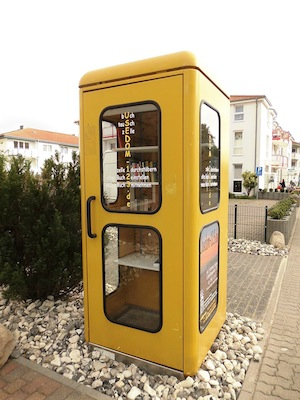
\includegraphics{img/BuchtauschzelleKarlshagen.jpg}
\caption{Bildunterschrift: CC-BY-3.0, Urheber: ChristianSW,
\url{https://commons.wikimedia.org/wiki/File:Buchtauschzelle_Karlshagen.jpg}}
\end{figure}

\section*{Variationen und
Weiterentwicklungen}\label{variationen-und-weiterentwicklungen}

\emph{Martin Clegg} und \emph{Michael Guttmann} haben viel mit der
\emph{Offenen Bibliothek} experimentiert. Eine besondere Umsetzung der
\emph{Offenen} \emph{Bibliothek} stellen die Installationen auf dem
\emph{Jüdischen Friedhof Krems} dar. Der Ort und seine Geschichte
bildeten hier die Grundlage für die inhaltliche Auswahl der
Buchbestände:

\begin{quote}
The Jewish cemetery in Krems has been unused since World War II.
\emph{The Open Public Library} in Krems is a revival project which will
give a reason and an opportunity for public access to one of the few
reminders that there was once a lively Jewish community in this Lower
Austrian city. {[}\ldots{}{]} The first bookcase contains original
religious material in Hebrew. The second cabinet contains introductory
material on Jewish law in German and English. The third part of the
collection specializes in various topics related to the Jewish
philosophy of death. (Clegg \& Guttmann: The Open Public Library in the
Jewish cemetary in Piaristenkirche Krems, In: Clegg \& Guttmann 2005, S.
96.)
\end{quote}

Spannend ist auch die Umsetzung des Projekts mit anderen Objektarten,
zum Beispiel Tonträgern oder Werkzeugen. Damit nähert sich die
\emph{Offene Bibliothek} der \emph{Givebox} an, bei der Gegenstände
aller Art abgelegt oder entnommen werden dürfen, aber nicht
zurückgebracht werden müssen.

Die Plattform \emph{OpenBookCase.org} verzeichnet \emph{Öffentliche
Bücherschränke}, \emph{Giveboxen} und vergleichbare Projekte mit
Geokoordinaten. Mit einem mobilen Endgerät lassen sich von jedem
Standort aus die in der Nähe gelegenen Objekte auf einer Karte anzeigen
und aufsuchen. So entsteht ein besonderes Verhältnis zwischen den
ortsgebundenen Objekten und ihrer öffentlichen Zugänglichkeit. Denkbar
wären weitere Verzahnungen zwischen den Projekten und dem Web 2.0,
beispielsweise eine Kennzeichnung der Bestände mit QR-Codes.

\newpage

\section*{Literatur}\label{literatur}

Clegg \& Guttmann (1990): Entwurf für eine \enquote{Open-Air}
Bibliothek, in: Durch 6/7 (1990), S. 136.

Clegg \& Guttmann (2005): Monument for historical change and other
social sculptures, community portraits and spontaneous operas. Wien :
Schlebrügge.Editor 2005.

Clegg \& Guttmann (1993): Offene Bibliotheken, in: Backstage. Topologie
zeitgenössischer Kunst. Hamburg : Kunstverein in Hamburg 1993, S. 10.

Kahle, Christian (2004): {[}Videozitat{]} Kommentiert -- 2004,
\url{http://bibliothekarisch.de/blog/2014/07/13/videozitat-kommentiert-2004/}

Könneke, Achim (Hg.) (1994): Clegg \& Guttmann. Die Offene Bibliothek.
The Open Public Library. Ostfildern : Cantz 1994.

Lingner, Michael (1993): Clegg \& Gutmanns »Offene Bibliothek«,
\url{http://ask23.hfbk-hamburg.de/draft/archiv/ml_publikationen/kt93-10.html}

Lingner, Michael (1991): «Metaphorische Selbstverwaltung»,
\url{http://ask23.hfbk-hamburg.de/draft/archiv/ml_publikationen/kt91-6.html}

%autor

\end{document}
